\documentclass[12]{article}
\usepackage{listings}
\usepackage[T1]{fontenc} 
\usepackage[utf8]{inputenc}
\usepackage[francais]{babel}
\usepackage{graphicx}
\usepackage{xcolor}

\definecolor{mGreen}{rgb}{0,0.6,0}
\definecolor{mGray}{rgb}{0.5,0.5,0.5}
\definecolor{mPurple}{rgb}{0.58,0,0.82}
\definecolor{backgroundColour}{rgb}{0.95,0.95,0.92}

\lstdefinestyle{CStyle}{
    backgroundcolor=\color{backgroundColour},   
    commentstyle=\color{mGreen},
    keywordstyle=\color{magenta},
    numberstyle=\tiny\color{mGray},
    stringstyle=\color{mPurple},
    basicstyle=\footnotesize,
    breakatwhitespace=false,         
    breaklines=true,                 
    captionpos=b,                    
    keepspaces=true,                 
    numbers=left,                    
    numbersep=5pt,                  
    showspaces=false,                
    showstringspaces=false,
    showtabs=false,                  
    tabsize=2,
    language=C
}

\title{Rapport Final}
\author{TM1G}

\begin{document}

\maketitle

\begin{abstract}
  Rapport Final du groupe TM1G de l'UE de Projet Technologique 2017 - 2018, composé de JEUNEHOMME Vincent, BERARDET Titouan, FURELAUD Thomas et GRIMARD Alan. \\
\begin{center}
  Chargé de TD: Monsieur BONICHON Nicolas
\end{center}
\end{abstract}

\tableofcontents



\section{Implémentation de la bibliothèque \textit{game}}
L'ensemble de l'implémentation de la bibliothèque game repose sur une structure de donnée représentant le jeu ainsi que les fonctions qui lui sont associées permettant au jeu de se dérouler.

De ce fait, nous verrons dans un premier temps la définition de cette structure, puis les différentes fonctions qui lui sont associées.
\subsection{La structure game}
\begin{lstlisting}[style=CStyle]
  struct game_s{
    int game_width;
    int game_height;
    int nb_ghost;
    int nb_vampire;
    int nb_zombie;
    int nb_spirit;
    content ** board;
    int ** labels;
  };
\end{lstlisting}

\subsection{Les énumérations utilisées}
 Les énumérations utilisées pour l'implémentation de la V1 (et de la V2) sont:
 -content : La liste des différents objets (les miroirs et les monstres) pouvant être présent dans le board de la game. On utilisera ce type fréquemment dans les fonctions modifiant le board.
 
 GHOST -> ne peut être vu qu'à travers un miroir.
 
     VAMPIRE -> ne peut pas être vu à travers un miroir.
     
     ZOMBIE -> est toujours vu.
     
     MIRROR -> redirige la ``ligne de vue'' arrivant selon l'orientation du miroir et la provenance de la ligne de vue. (/)
     
     ANTIMIRROR -> même utilité que pour le miroir mais dispose d'une orientation différente. 
 
 -direction : Est composée des quatre points cardinaux. Sera principalement utilisé en lien avec les labels.
 
\subsection{Les fonctions}
Chaque fonction implémentée dans game.c fait intervenir ou modifie les champs de la structure game.
\subsubsection{ Fonctions liées au champ board}
Les fonctions add\_mirror et add\_monster ajoutent une constante de type content aux coordonnées col et line dans le champ board de la game, un miroir pour add\_mirror et un monstre pour add\_monster.

  La fonction get\_content renvoie la constante de type content situé aux coordonnées col et line.

  Tandis que la fonction current\_nb\_monsters parcourt le board de game et renvoie le nombre d'occurrence du type de monstre demandé.
\subsubsection{ Fonctions liées au champ label}
La fonction set\_required\_nb\_seen change le label situé à la position pos et du coté side par exemple set\_required\_nb\_seen(game g, direction N, 0,4) va changer la valeur du premier label situé en haut par 4.

Tandis que required\_nb\_seen renvoie la valeur du label demandé.

La fonction current\_nb\_seen  est une sorte de ligne de vue qui compte le nombre de monstre vu depuis le label indiqué jusqu'à être hors du board. Pour cela, on parcourt le board via les variables vx et vy qui définiront dans quel sens aller (selon le label de départ, si le label est au nord on parcourt board de haut en bas), tout en utilisant une variable seenMirror qui indique si, sur la case où l'on est, il y a un miroir, dans le cas où il y a un miroir on utilise la fonction mirrorEncounter qui va changer vx et vy (par conséquent redirige la ligne de vue) selon le type de miroir indiqué.

Exemple:

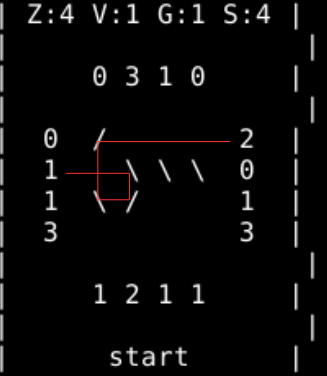
\includegraphics[height=5cm]{ex_ligne_de_vue.png}

Dans cet exemple, current\_nb\_seen(game, W, 1) part du second label à l'ouest et va parcourir le board selon la ligne rouge et compter le nombre de monstre visible.
\subsubsection{ Fonctions liées à toute la structure game}
La fonction new\_game va allouer l'espace mémoire nécessaire à une variable de type game puis aux champs labels et board, les autres champs seront initialisés à 0 (sauf pour game\_width et game\_height dont on traitera les cas dans la v2).

La fonction setup\_new\_game commence en appelant la fonction new\_game puis va modifier ses champs en fonction de ce qu'on lui a mit en paramètre, soit les nombres requis de chaque type de monstre, les labels ainsi que board (dans board on n'ajoutera que les content faisant référence à un mirroir en général).

copy\_game ce contente d'allouer tout l'espace nécessaire pour une game, ses labels et son board (dans cet ordre) puis va copier un à un tout les champs de la game rentrée en paramètre.

  delete\_game va libérer les espaces alloués, en premier lieu, au board, puis au champ labels et enfin à la structure game (ainsi on évite les fuites mémoires).

  restart\_game va parcourir le champ board et retirer tout ce qui n'est pas un miroir.

  Et enfin, la fonction is\_game\_over vérifie si les conditions de victoire sont réunis soit que :
  \begin{itemize}
  \item le nombre de monstre vu correspond aux labels (required\_nb\_seen est égal au label indiqué)
  \item le nombre de monstre présent dans la grille soit égal au nombre de monstre requis (current\_nb\_monster monster type == required\_nb\_monster monster type)
  \end{itemize}
  Si les conditions sont vérifiées, la partie est finie sinon elle continue.

  Exemple:

  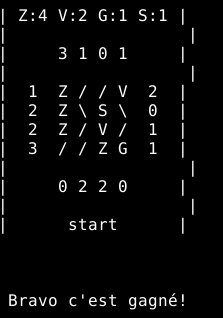
\includegraphics[height=5cm]{ex_is_game_over}

  Dans cet exemple, pour chaque label, si on effectue current\_nb\_seen le nombre renvoyé par la fonction est égale à celui indiqué par le label mis en paramètre. De plus le nombre de monstre de chaque type posé dans le board est égale au nombre requis de monstre de même type (indiqué par l'affichage Z:4 V:2 G:1 S:1) 
 \subsubsection{ Fonctions liées aux champs nb\_(ghost, zombie ou vampire)}
 set\_required\_nb\_monsters change le champ correspondant à la variable monster (de type content) (ex : change nb\_ghost si monster vaut GHOST)
 
 required\_nb\_monsters renvoie le champ correspondant au monstre rentré en paramètre (ex : renvoie la valeur de nb\_zombie si monster vaut zombie)


 Pas de difficulté notable rencontrée à cette étape.
\section{Adaptation de \textit{game} en v2}

\subsection{Ajout des fonctionnalités}
L'objectif de la V2 était de rajouter 1 type de monstre, 2 types de miroires et la possibilité de faire des grilles de taille variable.

Champs game\_width et game\_height -> contenant respectivement la largeur et la hauteur voulu pour la grille. Pour y accéder, nous avons dû implémenter les fonctions game\_width et game\_height.

SPIRIT -> type de monstre ne pouvant pas être vu

HMIRROR -> miroir horizontal. (-)

VMIRROR -> miroir vertical. (|)

new\_game\_ext -> a la même utilitée et fonctionnement que la fonction new\_game à ceci près qu'elle initialise les champs game\_width et game\_height selon les valeurs indiquées en paramètre.

setup\_new\_game\_ext -> a la même utilitée et fonctionnement que la fonction setup\_new\_game si ce n'est qu'elle appelle la fonction new\_game\_ext pour initialiser sa game de base.

add\_mirror\_ext -> pour déterminer le miroir à ajouter ont utilise plus de paramètre direction mais directement le type de miroir que l'on veut ajouter sur le board.

A noter que les homologues de ces fonctions moins le suffixe -ext appellent désormais ces fonctions en leur donnant des paramètres par défaut (ex new\_game appelle new\_game\_ext avec comme paramètre 4 pour la largeur et la hauteur).
\subsection{Modifications du code déjà existant}
Il a fallu rajouter dans l'énumération content SPIRIT, HMIRROR et VMIRROR.
Par conséquent, il a fallu changer les fonctions current\_nb\_seen (ainsi que la fonction associée mirrorEncounter), current\_nb\_monsters, set\_required\_nb\_monsters, required\_nb\_monsters et is\_game\_over afin de prendre en compte ces nouveaux type de content.


Pas de difficulté notable rencontrée à cette étape.
\section{Version texte du jeu}
\subsection{Synthèse du travail sur undead\_text.c}
\subsubsection{Fonctionnalités}
Par rapport aux fonctionnalités, cette version du jeu peut être lancée de deux façons différentes :
\begin{itemize}
\item soit en ne mettant aucun argument lors de l'exécution du fichier, ce qui lance alors une grille de jeu aléatoirement créée grâce à la fonction game\_alea. Cette fonction tire un nombre aléatoire, et place dans le contentboard soit rien, soit un monstre, soit un miroir suivant le nombre obtenu.
\item La deuxième façon de lancer cette version est de mettre un argument lors de l'exécution (comme 'game0') qui lancera alors la grille de jeu demandée si elle existe (retourne une erreur si la grille demandée n'existe pas).
\end{itemize}
  Une fois que le jeu est lancé on se retrouve donc directement dans la grille de jeu sans monstre. Ces derniers sont placés en tapant les coordonnées voulues puis le type de monstre que l'utilisateur souhaite placer. Si les coordonnées indiquées sont fausses (pas dans la grille ou sur un miroir par exemple) alors une nouvelle coordonnée est demandée.Si elle se trouve sur un monstre alors elle remplace le monstre présent par celui demandé par l'utilisateur.
  
  Lorsque le jeu est fini et que le joueur a la bonne combinaison(qu'il a gagné) un message de victoire s'affiche. Si il a rempli la grille mais que c'est faux alors le jeu continu.
\subsubsection{Code} 
Au niveau du code de cette partie on a tout d'abord deux énumérations : une qui contient tout ce qui peut être dans une case de la grille (vide, tout les types de miroirs et de monstres), et une autre pour la direction (Nord, sud, est et ouest).

Ensuite on a des fonctions pour définir les informations d'une grille, comme la largeur ainsi que la hauteur de la grille, mais aussi les labels, le nombre de monstres attendus dans la grille et ceux déjà présents dedans, ou encore pour 'demander' qu'est-ce qui se trouve dans une case dont on précise les coordonnées. On a aussi une fonction qui nous dit combien de monstres sont visible sur la ligne d'un label(donc pour voir si on a gagné ou pas) ou encore une fonction qui permet de rajouter un monstre ou un miroir dans la grille.

Pour finir on a codé des fonctions un peu plus général pour copier une grille de jeu à l'identique, ou encore une fonction qui nous dit si on a gagné, une qui efface la grille ou même une qui crée une grille avec des paramètres donné dans la fonction. Toutes ces fonctions nous permettent donc d'avoir une interface texte assez fonctionnelle, sans bug (du moins, découvert), et assez rapide.

Aucune grande difficulté n'a été rencontrée lors de la réalisation de cette étape. 

\section{Fonctionnement du solveur}
Le solveur que nous avons réalisé fonctionne en deux temps, premièrement il traite des données relatives à la game qu'il va ensuite, dans un second temps, utiliser lors de sa résolution de la game afin d'avoir un meilleur temps que de manière classique.

Ainsi, nous verrons brièvement le solveur en lui même, puis, plus en détail le fonctionnement permettant de préprocesser les données pour le solveur car c'est la partie la plus importante de ce solveur.


\subsection{Le solveur}
Le solveur en soit fonctionne bêtement, pour chaque case de la game il ajoute un monstre, si celui-ci n'invalide pas les propriétés de la game (required nb seen trop grand par exemple) alors il fait de même pour la case suivante, sinon, il essaye avec un monstre différent, et si pour une case, il a deja testé tous les monstres possibles, alors il revient en arrière et essaye avec un autre monstre.
\medbreak
A chacune de ces récursions (il fonctionne de manière récursive) le solveur vérifie si la condition game over est vraie (si il a trouvé une solution).
\medbreak
Selon le mode de jeu, si il trouve une solution il y a trois cas de figure:
\begin{itemize}
\item Mode de jeu FIND\_ONE, le solveur sauvegarde s'arrête.
\item Mode de jeu FIND\_ALL, le solveur sauvegarde et continue jusqu'à la dernière possibilité.
\item Mode de je NB\_SOL , le solveur continue mais au lieu de sauvegarder, il incrémente une variable qui compte le nombre de solutions.
\end{itemize}
\bigbreak

\subsection{la préparation du solveur}
Cette méthode de solveur seule fonctionne très bien certes mais cela nécessite de tester beaucoup trop de combinaisons dans certains cas, rendant le solveur très lent.
On peut représenter pour chaque case de la game, les possibilité de monstres qui lui sont associées par une liste de type content. Par exemple si pour une ligne de vue le label est 0, on peut en déduire que pour toutes le cases se trouvant sur cette ligne de vue, la liste de monstres possibles exclue le zombie, ou si ce même label est égal au nombre de cases sur la ligne de vue, on peut exclure toute possibilité de spirit dans la liste des possibilités de chaque case.
\medbreak
Nous allons représenter l'ensemble des listes de possibilités par une liste de liste de liste de content (content en 3D)
ainsi, chaque case de ce tableau de content correspondra à la liste de monstres que le solveur pourra placer.

\begin{lstlisting}[style=CStyle]
  content *** ordre;
\end{lstlisting}
\medbreak
La fonction déduction initialisera cette matrice à la liste par defaut contenant (ZOMBIE,GHOST,VAMPIRE,SPIRIT), puis en appelant la fonction parkour depuis chaque case de bordure de chaque direction, parkour récoltera des information telles que l'historique des cases traversées, la longueur de la ligne de vue, si un miroir à été traversé, si on a effectué un demi-tour.
Ces information que parkour a récolté, seront transmises à la fonction aply, qui elle selon ces données retirera de la liste des possiblités les monstres correspondants à des cas impossibles (codées en dur dans la fonction) sur tout l'historique des cases parcourues.

A partir de là, les possibilités sont en général conidérablement amoindries, cependant, dans les cas ou la game devient excessivement grande, et qu'elle dispose de beaucoup de solutions, cela n'aidera pas le solveur à aller plus vite.
\section{Version graphique du jeu}
\subsection{Synthèse du travail sur la version graphique}
\subsubsection{Au niveau du code}
Dans cette partie on va tout d'abord vous parlez du fichier model.c.

Tout d'abord nous avons créé deux énumérations et trois structures. Les énumérations sont:
\begin{itemize}
\item pour l'action qui est demandée lorsqu'on appuie sur un bouton (select zombie, do quit, ...)
\item et la deuxième sert à savoir où on se trouve dans le jeu(MENU(menu de départ), HELP(menu howtoplay), ...).
\end{itemize}
Quant aux structures :
\begin{itemize}
\item la première est pour les boutons(coordonées en haut à gauche, dimensions, quelle action fait ce bouton, le text qu'il contient,...),
\item la deuxième est pour les coups(la position dans la grille et le monstre qu'on pose)
\item et enfin la dernière pour l'environnement(la où on va venir déclarer toutes les choses dont on va avoir besoin dans notre interface graphique).
\end{itemize}

Ensuite on a créé différentes fonctions \textit{'load'} pour tout les sous menus qu'on rencontre dans notre jeu avec les différents background de ces derniers ainsi que leurs boutons et leurs emplacements(Par exemple \textit{loadplayground} qui contient tout les boutons des monstres, ainsi que le background qui se trouve derrière la grille de jeu et les textes sur les boutons).Pour chaque sous-menus il existe une unique fonction \textit{load}.


Pour les boutons présents dans notre jeu on a créé cinq fonctions. La premiere étant \textit{setBouton} qui, comme son nom l'indique, crée un nouveau bouton.\textit{SetBouton} a pour paramètre les coordonnées du bouton ainsi que sa dimension, mais aussi son action, et le texte inscrit dans celui-ci. Ensuite on a une fonction \textit{actualizeButton} qui actualise la taille du bouton quand la fenêtre change de dimension.
On a aussi la fonction \textit{isPushed} qui regarde si on clique actuellement sur un bouton par rapport aux coordonnées de la souris ainsi que la fonction \textit{click} qui nous dit quoi faire qand on clique sur un bouon (revenir au menu, poser un monste, selectionner un monstre,...).
Pour finir on a la fonction \textit{putMonster} qui pose le monstre sélectionné aux coordonnées de la souris.

\subsubsection{Au niveau graphique}

D'un point de vue graphique, on a ensuite reprit la fonction \textit{Init} qui crée un environnement et qui charge toutes les images dont on va avoir besoin dans notre jeu ainsi que notre position de départ (dans le menu). On prend aussi les dimensions de la fenêtre.
Par la suite on a reprit encore une fois la fonction \textit{render} du demo.c pour faire l'affichage de notre jeu. On initialise donc le background de notre jeu, mais aussi les boutons ainsi que les écriture sur ces derniers. On affiche aussi les labels ainsi que quelques lignes dans cette fonction.

Pour finir on a le \textit{clean} qui détruit toutes les textures ainsi que la grille de jeu et tout les boutons.

Grâce à toutes ces fonctions lorsqu'on lance le jeu on se retrouve sur une interface avec 4 boutons : play, load, howtoplay et quit. Le play lance la dernière game qui a été lancée (ou la game0 par défaut). Le load lance un nouveau menu avec 3 boutons : game0, random, et retour. Et pour finir howtoplay nous indique comment jouer et grâce à quit on quitte le jeu.

\subsubsection{Au niveau des fonctionnalités}
Au niveau des fonctionnalités de notre jeu, Vincent a créé une fonction undo qui permet d'annuler les coups précédemment joué. On a aussi une fonction qui crée une grille de jeu aléatoire comme pour undeadtext. Ensuite on a un bouton 'solution' au dessus de notre grille de jeu pour résoudre la grille et la montrer à l'utilisateur à sa demande.
Le fait de créer un nouveau sous-menu avec des grilles aléatoires de différentes tailles aurait pu être une fonctionnalité à rajouter. 


\section{Les Tests}
\subsection{Démarche de test}
L’élaboration d’une procédure de test est primordiale dans un projet tel que celui-ci. Cette procédure nous permet de pouvoir vérifier que nos fonctions font bel et bien la ou les tâches qu’elles sont censées faire. Ainsi, on s’assure de ne pas brûler les étapes : on ne s’autorise à utiliser les fonctions dans notre programme uniquement si elles sont testées et validées. De cette manière, lorsque nous tombons sur des erreurs dans notre programme, on arrive beaucoup plus facilement à cerner d’où exactement vient le problème, et à le corriger.\\ 

Les tests sont, de manière globale, du code très simple : on exécute la fonction à tester, puis on analyse se qu’elle retourne, ou l’action qu’elle a effectué. On renvoi un booléen en fonction du résultat de l’analyse : true la fonction fonctionne, false elle ne fonctionne pas. Pour que cette procédure de test fonctionne, il faut s’assurer que le test exécute et analyse toute les possibilités imaginables.\\ 

	Les tests doivent évidemment être modifiés si les fonctions ont, après modifications, de nouvelles fonctionnalités. Typiquement, lorsque nous sommes passés de la V1 à la V2, qui a entraîné l’ajout de nouveaux monstres et miroirs, les tests des fonctions current\_nb\_seen et current\_nb\_monster par exemple ont également dû être modifiés pour tester les fonctions sur les nouveaux types de monstres et miroirs.
\subsection{Tests sur les fonctions dites "simples"}
Dans un premier temps, une fois les fonctions dites « simples » (c’est à dire qui exécutent des tâches simple sans faire intervenir d’autres fonctions) écrites, tel que add\_monster, set\_required\_nb\_seen, ou get\_content,  on écrit et exécute les tests correspondant à ces fonctions.\\
	
Voici un exemple avec la fonction get\_content :
\begin{lstlisting}[style=CStyle]
content get_content(cgame game, int col, int line){
    if(game==NULL){
        fprintf(stderr,"pointeur null\n");
        exit(EXIT_FAILURE);
    }
    return game->board[col][line];
}
\end{lstlisting}

Pour se faire, nous avons créé une game à la main, à l’aide des fonctions add\_monster et add\_mirror\_ext, préalablement testées:

\begin{lstlisting}[style=CStyle]
bool test_get_content(){

    printf("testing get_content()             : ");
    bool res=true;
    game g = new_game();
    assert(g);

    /*
    | Z:1 V:1 G:1 S:1 |
    |                 |
    |     X X X X     |
    |                 |
    |  X  Z   - \  X  |
    |  X  V   / |  X  |
    |  X  G        X  |
    |  X  S        X  |
    |                 |
    |     X X X X     |
    |                 |
*/

    add_monster(g, SPIRIT, 0, 0);
    add_monster(g, GHOST, 0, 1);
    add_monster(g, VAMPIRE, 0, 2);
    add_monster(g, ZOMBIE, 0, 3);

    add_mirror_ext(g, MIRROR, 2, 2);
    add_mirror_ext(g, ANTIMIRROR, 3, 3);
    add_mirror_ext(g, VMIRROR, 3, 2);
    add_mirror_ext(g, HMIRROR, 2, 3);
\end{lstlisting}

Nous avons ensuite vérifié, pour chaque types de cases (monstres, miroirs et cases vides) que l’appel à la fonction get\_content(g, x, y) nous donnait bien le bon type content de la case en sortie :
\begin{lstlisting}[style=CStyle]
    if(get_content(g, 0, 0) != SPIRIT) {
        if(res==true){
            printf("Basic test on get_content failed\n");
        }
        printf("	|content of value : SPIRIT : should have been detected but have not\n");
        res=false;
    }

    if(get_content(g, 0, 1) != GHOST) {
        if(res==true){
            printf("Basic test on get_content failed\n");
        }
        printf("	|content of value : GHOST : should have been detected but have not\n");
        res=false;
    }
\end{lstlisting}

Enfin, on supprime proprement la game créée, puis on retourne le booléen :

\begin{lstlisting}[style=CStyle]
    delete_game(g);
    if(res==true){
        printf("ok.\n");
    }

    return res;
}
\end{lstlisting}

La procédure est quasiment la même pour toutes les fonctions.\\

Certaines fonctions de test ont dû utiliser l’outil Valgrind pour analyser les fuites mémoires éventuelles suite à l’appel d’une fonction.
\subsection{Tests sur les fonctions dites "complexes"}
On s’assure que ces fonctions simples fonctionne parfaitement pour ensuite tester des fonctions plus complexe (comme new\_game\_ext), qui utilisent une ou plusieurs de ces mêmes fonctions simples ( game\_width et game\_height pour cet exemple).\\

Pour se faire, il nous faut veiller à l’ordre des tests des fonctions. En effet, pour tester une fonction X qui utilise une ou plusieurs fonctions Y, il nous faut logiquement tester en premier les fonctions Y avant de tester la fonction X. De cette manière, il nous sera mis en évidence beaucoup plus facilement si une erreur viens de la fonction X, ou des fonctions Y qu’elle utilise.\\

La procédure de test est la même que pour les fonctions « simples ».

\subsection{Test du solveur}

Le solveur, élément clé du projet, a été plutôt simple à tester dans notre cas. Dans un premier temps, nous avons initialisé une grille à la main :

\begin{lstlisting}[style=CStyle]
bool test_solveur(){
    bool res = true;
    printf("testing solveur()    	          : ");
    int width = 4;
    int height = 4;
    game g = new_game_ext(width, height);
    /* Map used in test_is_game_over function (solution map only)
    | Z:3 V:2 G:2 S:2 | Z:3 V:2 G:2 S:2 |
    |                 |                 |
    |     0 1 3 2     |     0 1 3 2     |
    |                 |                 |
    |  0  \     |  0  |  0  \ V V |  0  |
    |  2  -        2  |  2  - S Z Z  2  |
    |  2      \ /  0  |  2  Z G \ /  0  |
    |  0  \     \  0  |  0  \ S G \  0  |
    |                 |                 |
    |     0 1 2 4     |     0 1 2 4     |
    |                 |                 |
    |     start       |     solution    |
*/

    int nb_ghosts = 2;
    int nb_vampires = 2;
    int nb_zombies = 3;
    int nb_spirits = 2;
    content board []={ANTIMIRROR, EMPTY, EMPTY, ANTIMIRROR, EMPTY, EMPTY, ANTIMIRROR, MIRROR, HMIRROR, EMPTY, EMPTY, EMPTY, ANTIMIRROR, EMPTY, EMPTY, VMIRROR};
    int North_labels [] = {0, 1, 3, 2};
    int South_labels [] = {0, 1, 2, 4};
    int East_labels [] = {0, 0, 2, 0};
    int West_labels [] = {0, 2, 2, 0};
    int *labels [] = {North_labels, South_labels, East_labels, West_labels};
    g = setup_new_game_ext(width, height, labels, board, nb_ghosts, nb_vampires ,nb_zombies, nb_spirits);
\end{lstlisting}

Nous avons ensuite initialisé tout les paramètres du solveur, puis appelé la fonction sur la game:

\begin{lstlisting}[style=CStyle]
    function fun = FIND_ONE;
    char * c = "solution";
    int k =0;
    unsigned int l=0;
    bool drop = false;
    content *** grid;
    grid = deduction(g);
    int tab[4]={0,0,0,0};
    solveur(&fun,g,c,&k,&l,&drop,grid,tab);
\end{lstlisting}
       
Nous avons écrit à la main dans le fichier « solution\_vrai.sol » la solution calculée à la main. Nous chargeons ensuite la solution du solveur (écrite dans le fichier « solution.sol »), et la solution calculée à la main dans deux games différentes. Enfin, nous vérifions que chaque cases de la solution calculée et la solution du solveur soient identique :

\begin{lstlisting}[style=CStyle]
    game g_correct = load_game("solution_vrai.sol");
    game g2=load_game("solution.sol");

    for (int i =0; i<width; i++){
        for (int j = 0; j<height; j++){
            if(get_content  (g_correct, i, j) != get_content(g2, i, j)){
                printf("Basic test on test_solveur failed\n	|return different than what was given\n");
                res = false;
                return res;
            }
        }

        /*content get_content(cgame game, int col, int line)*/
    }
    printf("ok.\n");
    return res;

}
\end{lstlisting}

\subsection{Bilan}

\subsubsection{Analyse}

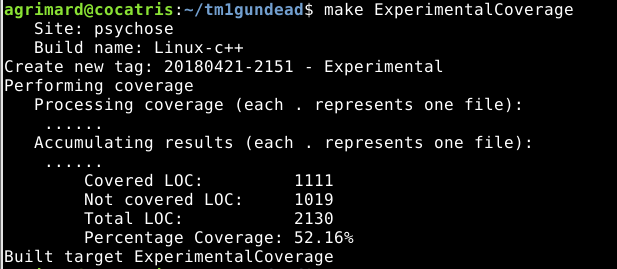
\includegraphics[height=5cm]{gcov}

Ce faible résultat (52,16\%) sur gcov trouve trois explications:
\begin{itemize}
\item nous n’avons pas testé toutes les fonctions qui utilisent la bibliothèque SDL. En effet, ces fonctions produisant uniquement des résultats visuels, nous n’avons pas trouvé de solution pour tester de manière automatique ces résultats.
\item nous n’avons pas testé les fonctions d’affichage de undead\_text, car nous n’avons pas su comment tester les printf fait sur la console.
\item certaines fonctions n'ont pas été testées sur la fin du projet.
\end{itemize}

\subsubsection{Difficultées et piste d'amélioration}
Ce processus de test n’est pas devenu tout de suite un automatisme pour nous. Bien que crucial, il fût mis de coté sur la fin du projet, par manque de temps principalement. C’est un risque que nous avons pris, et que nous assumons pleinement. C’est une de nos principales erreurs, et nous avons compris l’importance d’une procédure de test solide : nous veillerons dorénavant à mettre une procédure de test de manière automatique et efficace pour nos futurs projets.



\section{Critiques de l'UE Projet Technologiques}
\subsection{Titouan}
Globalement, je pense que l'UE est très bien. On commence par des choses simples et guidées puis la difficulté augmente progressivement. Les étudiants doivent travailler de façon autonome. Les enseignants sont à l'écoute et donnent des pistes intéressantes aux groupes en difficultés sans pour autant faire le travail à leur place. Le nombre de TD était, à mon avis, suffisant et les délais raisonnable. Cependant certains outils auraient pus être donné plus tôt (je pense notemment à qtcreator ou bien gcov) ou bien avoir un cours magistral afin de mieux expliquer leurs fonctionnalités et appuyer sur leur importance.

En conclusion, l'UE rempli son objectif mais devrait donner de meilleures habitudes aux étudiants tel qu'utiliser un éditeur de texte plus complet que gedit.

\subsection{Thomas}
Pour ma part j'ai trouvé cette UE très enrichissante. Celle-ci m'a apprit à mieux coder en C et à plus réfléchir quand j'écris un programme. Je trouve que cette UE est vraiment d'une grande aide pour les étudiants comme moi qui ne trouvent pas forcément le plaisir d'apprendre par coeur des cours en C (comme l'UE programmation C), au contraire celle-ci nous fait apprendre par nous-même (dans des délais respectables) et avoir un but m'a, personnellement, motivé. Ensuite il est vrai que quand on a une personne comme Vincent dans son groupe, ça aide, car quand on ne savait pas faire quelque chose ou qu'on avait une erreur dans notre code, il nous épaulait vraiment bien.

Pour conclure, je trouve cette UE vraiment enrichissante à tout niveaux (travail en groupe, apprentissage du C et de nouveaux outils(git, qtcreator,...)).

\subsection{Alan}
Cette UE est de loin celle qui nous aura demandé le plus gros volume de travail. Mais c’est également celle qui est la plus intéressante, puisqu’elle nous propose de mettre en œuvre un projet concret, de manière très bien encadrée par nos chargés de TD.

Personnellement, étant donné que je me dirige absolument pas vers un projet professionnel en rapport direct avec la programmation pure, mais plutôt vers de la gestion d’équipe et de projet, seul l’aspect « gestion de projet », les outils proposés (gcov, git…) et la méthodologie de projet m’ont intéressés. Le projet en lui même ne m’intéressait pas vraiment, mais uniquement parce que la programmation de jeu en elle même ne m’intéresse pas vraiment.

\subsection{Vincent}
Ce projet m'a énormément fait progresser en programmation c ce semestre, il m'a permis de bien apprendre la synthaxe, de comprendre l'allocation dynamique et de mettre en application tout ce qu'on a vu en cours. Comparer mes compétences entre pendant et après ce troisième semestre, c'est le jour et la nuit. Le déroulement de l'UE s'est trés bien passé, je pense que le découpage du projet en plusieurs phases était réussi. Les outils de développement vus sont très utiles et pertinents pour le projet, bien que je ne comprenne pas encore le fonctionnement de git sur certains aspects (branches), coder en parallèle est pratique, mais on se heurte parfois à des erreurs où l'on ne sait pas quoi faire (lors des merge notamment). Je pense qu'il eut été bien de passer peut être un peu plus de temps sur cet outil en TD machine.


\end{document}

